\section{寄存器描述}
\regover{
{\hyperref[kys-ks-ctrl]{ks\_ctrl}}&Keyscan contro
\\
\hline
{\hyperref[kys-ks-int-en]{ks\_int\_en}}&Keyscan interrupt enable
\\
\hline
{\hyperref[kys-ks-int-sts]{ks\_int\_sts}}&Keyscan interrupt status
\\
\hline
{\hyperref[kys-keycode-clr]{keycode\_clr}}&Keycode clear
\\
\hline
{\hyperref[kys-keycode-value]{keycode\_value}}&Keycode value
\\
\hline
}

\subsection{ks\_ctrl}
\label{kys-ks-ctrl}
地址:0x4000a900
 \begin{figure}[H]
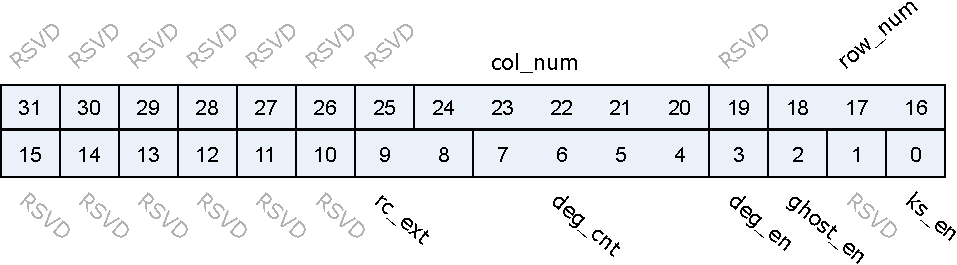
\includegraphics{kys_ks_ctrl.pdf}
\end{figure}

\regdes{31:25&RSVD& & & \\\hline
24:20&col\_num&r/w&5'd19&col\_num + 1\\\hline
19&RSVD& & & \\\hline
18:16&row\_num&r/w&3'd7&row\_num + 1\\\hline
15:10&RSVD& & & \\\hline
9:8&rc\_ext&r/w&2'd3&idle duration between column scans\\\hline
7:4&deg\_cnt&r/w&0&\\\hline
3&deg\_en&r/w&0&deglitch\\\hline
2&ghost\_en&r/w&0&ghost key event detection\\\hline
1&RSVD& & & \\\hline
0&ks\_en&r/w&0&\\\hline

}
\subsection{ks\_int\_en}
\label{kys-ks-int-en}
地址:0x4000a910
 \begin{figure}[H]
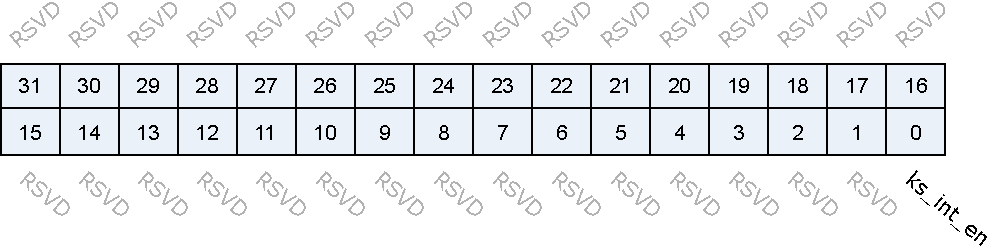
\includegraphics{kys_ks_int_en.pdf}
\end{figure}

\regdes{31:1&RSVD& & & \\\hline
0&ks\_int\_en&r/w&1&\\\hline

}
\subsection{ks\_int\_sts}
\label{kys-ks-int-sts}
地址:0x4000a914
 \begin{figure}[H]
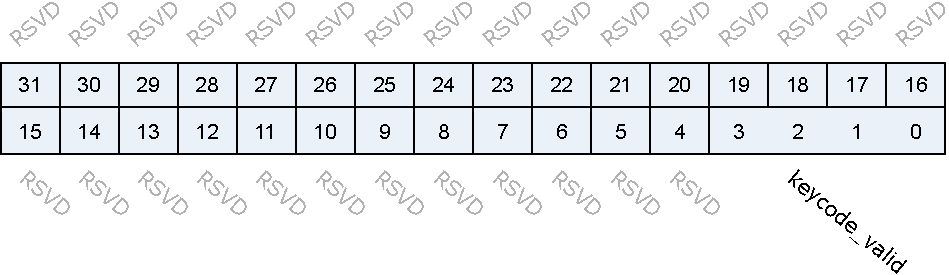
\includegraphics{kys_ks_int_sts.pdf}
\end{figure}

\regdes{31:4&RSVD& & & \\\hline
3:0&keycode\_valid&r&0&\\\hline

}
\subsection{keycode\_clr}
\label{kys-keycode-clr}
地址:0x4000a918
 \begin{figure}[H]
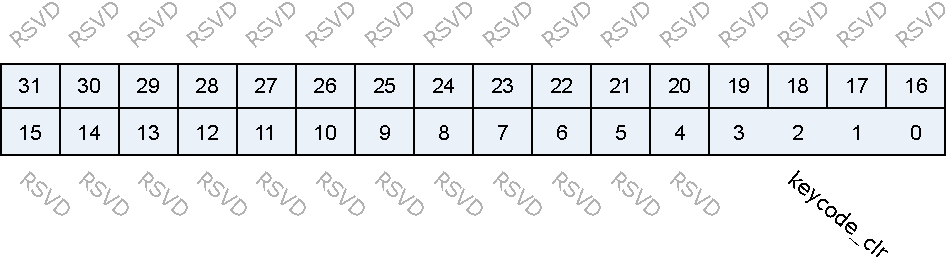
\includegraphics{kys_keycode_clr.pdf}
\end{figure}

\regdes{31:4&RSVD& & & \\\hline
3:0&keycode\_clr&w1c&0&\\\hline

}
\subsection{keycode\_value}
\label{kys-keycode-value}
地址:0x4000a91c
 \begin{figure}[H]
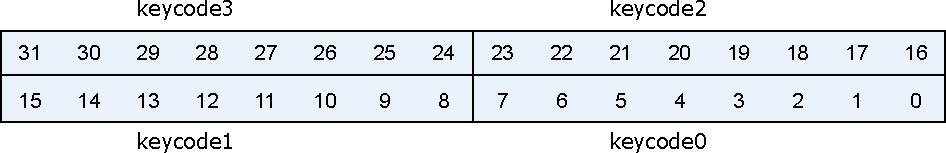
\includegraphics{kys_keycode_value.pdf}
\end{figure}

\regdes{31:24&keycode3&r&8'hff&\\\hline
23:16&keycode2&r&8'hff&\\\hline
15:8&keycode1&r&8'hff&\\\hline
7:0&keycode0&r&8'hff&Col = keycode / (row\_num+1) \par Row = keycode % (row\_num+1)
\\\hline

}
